
\title{Диагностика ошибок при анализе встроенных языков}
%
\titlerunning{Диагностика ошибок при анализе встроенных языков}

\author{Вербицкой Екатерина Андреевна}
%
\authorrunning{Е.А.Вербицкая} % abbreviated author list (for running head)
%
%%%% list of authors for the TOC (use if author list has to be modified)
\tocauthor{Е.А.Вербицкая}
%
\institute{Санкт-Петербургский государственный университет\\
\email{kajigor@gmail.com}}

\maketitle              % typeset the title of the contribution

\section*{Введение}
Несмотря на развитие техник метапрограммирования, порождающего программирования 
(generative programming) и ORM-технологий, использование в языках программирования 
динамически формируемых строковых выражений все еще широко распространено. 
Примерами могут служить динамические SQL-запросы к базам данных в java-коде и 
динамическое формирование HTML-страниц. Во время разработки программного обеспечения
с использованием встроенных языков возникает множество проблем, связанных с тем, 
что такой код статически не анализируется, и поэтому об ошибках становится 
известно лишь во время выполнения. В худшем случае ошибка не приведет к прекращению 
работы приложения (это явно бы указало на проблемы), но при этом консистентность 
данных может оказаться нарушена. Динамически формируемые выражения, по сути, являются 
результатом конкатенации строк исходного языка в циклах или внутри веток условных 
операторов, причем эти структуры могут вкладываться друг в друга, что создает 
множество различных вариаций, каждая из которых потенциально содержит ошибки. 
Для упрощения процесса разработки и отладки приложений, написанных с использованием 
встроенных языков, оказываются полезными инструменты, проводящие анализ множества 
выражений, которые могут быть получены на этапе исполнения из строковых выражений 
исходного языка. Будем называть данный процесс статическим анализом динамически 
формируемых выражений.

В рамках исследовательского проекта YaccConstructor~\cite{YaccConstructor}, посвященного проведению 
экспериментов в области синтаксического анализа, ведется работа над платформой 
для создания инструментов, предназначенных для статического анализа кода на встроенных
языках. В ходе работы над проектом были реализованы алгоритмы абстрактного 
лексического и синтаксического анализа~\cite{grigorev2013glr}. “Абстрактный анализ” в данном контексте 
означает, что анализатор принимает на вход не линейный поток, а некоторую более 
сложную структуру данных. За основу реализованного абстрактного синтаксического 
анализатора взят RNGLR-алгоритм анализа~\cite{Scott:2006:RNG:1146809.1146810}, модифицированный таким образом, чтобы 
принимать на вход вместо потока токенов некоторый граф.

Несмотря на то, что абстрактный GLR-алгоритм, во многом, схож с классическим~\cite{grigorev2013glr}, 
механизм диагностики и обработки ошибок нуждается в существенной доработке. 
Наивное переиспользование алгоритма обнаружения ошибок в  абстрактном синтаксическом 
анализе приводит к тому, что действительные ошибки во встроенном коде могут 
восприниматься как ошибки синтаксического анализа, и поэтому игнорироваться. 
Однако такие ситуации представляют непосредственный интерес для конечного пользователя 
инструмента, поэтому не должны быть пропущены. 

В данной работе исследованы особенности обнаружения ошибок в алгоритме абстрактного 
синтаксического анализа, основанного на GLR-алгоритме. Выявлен ряд недостатков 
ранее реализованного алгоритма, часть из которых удалось решить. Также описаны 
проблемы, вызванные спецификой базового алгоритма, решить которые не удалось. 

\section{Обзор}
Для обработки встроенных языков в статье Kyung-Goo Doh, Hyunha Kim и David A. 
Schmidt~\cite{Doh:2011:AL:2074591.2074599} был предложен алгоритм абстрактного 
синтаксического анализа, основанного на LR-алгоритме. Использование LR-алгоритма
вводит ограничения на класс обрабатываемых грамматик. В рамках проекта 
YaccConstructor ведется разработка платформы для создания инструментов, 
предназначенных для статического анализа кода на встроенных языках. Разрабатываемая 
платформа получила название AbstractYaccConstructor (AYC). Для того чтобы 
воспользоваться преимуществами обобщенного LR-алгоритма (GLR) как алгоритма 
синтаксического анализа, в рамках платформы AYC именно GLR взят за основу алгоритма 
абстрактного синтаксического анализа. 

\subsection{Описание платформы AbstractYaccConstructor}
Платформа AYC создана как часть проекта YaccConstructor и использует его идеи 
модульности и возможности использования языков спецификации грамматик. Абстрактный
статический анализ проводится по шагам: сначала проводится аппроксимация множества 
значений динамически формируемого выражения, далее проводится лексический, а затем
синтаксический анализ. Лексический и синтаксический анализаторы генерируются по 
лексической спецификации и грамматике языка. Модульность инструмента позволяет 
далее проводить другие виды анализа, например семантический или анализ типов. 
Далее шаги статического анализа описаны подробнее. 

Первым шагом проводится аппроксимация множества значений динамически формируемого 
выражения. Для этого проводится протягивание констант, при этом конкатенация в циклах 
заменяется на единственное повторение. В результате формируется ориентированный 
ациклический граф (directed acyclic graph, DAG), содержащий на своих дугах 
фрагменты строковых выражений из исходного кода. 

Далее полученный граф передается на вход абстрактному лексеру, сгенерированному 
по лексической спецификации встроенного языка. Абстрактный лексер производит 
анализ и формирует так же ориентированный ациклический граф, на дугах которого
содержатся токены, соответствующие входу. Также сохраняется привязка к исходному 
коду, чтобы в дальнейшем можно было производить позиционирование в исходном коде, 
необходимое для подсветки синтаксиса, сигнализации об ошибках. 

На следующем шаге граф, содержащий результаты абстрактного лексического анализа 
передается абстрактному синтаксическому анализатору. В качестве основы абстрактного 
синтаксического анализатора выбран RNGLR-алгоритм (улучшение оригинального GLR-алгоритма, 
отличающееся в основном способом генерации LR-таблиц). Результат, полученный на 
этом шаге может использоваться для проведения дальнейших шагов анализа, вычисления 
семантики, или же для простой подсветки синтаксиса и сигнализации об ошибках, 
если таковые присутствуют.

\subsection{Описание GLR-алгоритма синтаксического анализа}
Существует множество алгоритмов анализа, каждый из которых накладывает ограничения 
на грамматику обрабатываемого языка. Чтобы расширить класс принимаемых анализатором
грамматик до класса неоднозначных контекстно свободных грамматик, был создан 
обобщенный восходящий магазинный анализатор (Generalized Left-to-right Rightmost,
GLR)~\cite{Tomita:1985:EPN:537456}. Используемые алгоритмом таблицы напоминают аналогичные таблицы для просто 
LR-алгоритма, только могут содержать более одного возможного действия для любого 
состояния и входного символа. Такие ситуации принято называть конфликтами. Они 
бывают двух видов: Shift/Reduce~— возможно либо взять новый токен для анализа,
либо произвести свертку стека; и Reduce/Reduce~— существует более одной возможности 
произвести свертку стека. 

GLR-анализатор оперирует с более сложной структурой данных, нежели классический 
LR-анализатор: со структурированным в виде графа стеком (Graph Structured Stack, GSS). 
В дальнейшем будем называть эту структуру данных просто стеком.  В случае возникновения 
конфликта следующее действие анализатора приводит к разветвлению стека, а в случае 
возникновения на вершинах двух ветвей одинаковых состояний, эти ветви склеиваются.
Таким образом избегается экспоненциальный взрыв по памяти и времени. В RNGLR-алгоритме 
вместо классических стековых операций переноса (shift) и перехода в следующее состояние 
(goto) введена новая операция push. Данная операция производит вычисление состояния 
LR-автомата и записывает соответствующую информацию на стек. 

Алгоритм работы со стеком имеет в основе поиск в ширину. Очередная операция push 
происходит только тогда, когда все остальные возможные операции выполнены. Таким 
образом, можно говорить о том, что стек изменяется уровнями, где уровни в RNGLR 
соответствуют номерам токенов в последовательном входе. Набор верхушек стека, для 
которых возможен дальнейший анализ, называется фронтом. Если для некоторой верхушки 
стека не существует ни одного возможного действия, она исключается из фронта. В 
классическом RNGLR-анализе все верхушки стека, принадлежащие фронту, лежат на одном 
уровне.

Так как GLR-алгоритм способен работать с неоднозначными грамматиками, то в результате 
его работы может быть получено более одного дерева разбора. Аналогично для того, 
чтобы избежать экспоненциального роста потребляемых ресурсов, для хранения леса 
разбора используется специальная структура данных — сжатое представление леса разбора 
(Shared Packed Parse Forest, SPPF~\cite{rekers1992parser}). 

\subsection{Особенности реализации абстрактного синтаксического анализатора}
Классический GLR-алгоритм синтаксического анализа, предложенный Томитой~\cite{Tomita:1984:LPN:980431.980564, Tomita:1985:ECP:1623611.1623625, Tomita:1985:EPN:537456}, 
все же накладывает ограничения на грамматику. Поэтому в рамках платформы YaccConstructor 
ранее был реализован не он, а RNGLR-алгоритм, описанный в работе~\cite{Scott:2006:RNG:1146809.1146810}. Главной 
особенностью RNGLR-алгоритма является особый способ построения LR-таблиц. 
RNGLR-алгоритм синтаксического анализа способен работать с произвольными контекстно 
свободными грамматиками. Именно этот алгоритм и был в дальнейшем взят за основу 
алгоритма абстрактного синтаксического анализа. 

Абстрактный синтаксический анализ вместо линейного потока токенов принимает на 
вход некоторый граф, на ребрах которого содержится информация о токене и служебная 
информация, необходимая для дальнейшего позиционирования в исходном тексте 
анализируемой программы. Разветвления во входном графе напоминают классические 
конфликты GLR-алгоритма: перед анализатором стоит выбор между переносом различных 
токенов с разных ребер. Такую ситуацию мы будем по аналогии называть Shift/Shift 
конфликтом, хоть она и не является конфликтом в классическом понимании этого термина. 
Shift/Shift конфликты обрабатываются аналогично классическим конфликтам GLR-алгоритма, 
при их возникновении происходит ветвление стека.

Как уже было сказано, входной структурой данных для абстрактного синтаксического 
анализа является ориентированный ациклический граф. В случае, когда входная структура 
алгоритма синтаксического анализа является направленным ациклическим графом, задача 
поиска неподвижной точки сводится к задаче обработки вершин графа в порядке 
топологической сортировки. Поэтому в нашей реализации входной граф представляется 
в виде списка вершин, отсортированных в топологическом порядке. Во время анализа 
для каждой вершины рассматриваются все исходящие ребра и для каждого ребра 
совершается операция push на стек (вычисляется состояние LR-автомата и соответствующая 
информация записывается на стек). Каждой операции push присваивается номер, равный
номеру конца дуги в топологической сортировке. Первым из ребер, исходящих из данной 
вершины, обрабатывается ребро, номер операции push которой минимален. Остальные 
ребра откладываются для дальнейшего анализа. 

В случае абстрактного синтаксического анализа уже нельзя сказать, что весь фронт 
находится на одном уровне. Верхушки стека, соответствующие отложенным операциям 
push, не изменяются до момента, пока анализ текущей ветви прекратится. После этого 
анализ продолжается для одной из отложенных операций push, при этом во фронте 
оказываются как верхушки для ранее разобранной ветви, так и текущие, лежащие уже 
на другом уровне верхушки.


\section{Особенности обнаружения ошибок в абстрактном GLR-анализе}
Первоначальная реализация механизма обнаружения ошибок в алгоритме абстрактного 
синтаксического анализа содержала множество недостатков, связанных как с переходом 
от классического анализа к абстрактному, так и характерных непосредственно для 
базового GLR-алгоритма. Далее будут описаны выявленные проблемы, а так же предложены 
шаги предпринятые для их решения.

\subsection{Проблемы первоначальной реализации}
Первоначальная реализация абстрактного GLR-анализатора по части обнаружения ошибок 
мало отличалась от классического GLR-анализатора. Классический GLR-анализатор 
перебирает все возможные варианты разбора, ветвя стек, при этом если на каком-то 
пути в графе синтаксический анализатор получил ошибочное  состояние, соответствующая 
ветвь стека считается ошибочной и целиком отбрасывается. Если все пути ведут в 
ошибочные состояния, тогда считается, что входная строка содержит ошибку. При этом 
происходит сигнализация только о последней (или первой, в зависимости от конкретного 
алгоритма) найденной в ходе разбора ошибке. 

Аналогичное поведение было и у первоначальной версии реализованного в рамках 
платформы AYC абстрактного синтаксического анализатора. Описанная базовая логика 
поиска ошибки была расширена правилом, согласно которому, если для данной дуги 
входного графа не получается найти ни одного правила, не приводящего к переходу 
к ошибочному состоянию, данная ситуация считается ошибкой. В этом случае абстрактный 
синтаксический анализатор возвращал результат разбора, соответствующий ошибке 
(Error), при этом разбор входного графа прекращался. Данное поведение приводило 
к игнорированию всех еще не разобранных путей в графе, соответствующих как ошибочным, 
так и корректным выражениям. 

После возникновения ошибочной ситуации вызывалась функция сбора информации об 
ошибке, необходимая для указания ошибочного токена, а так же его позиции в исходном 
коде. Данная функция анализировала стек и, если находила на одном уровне стека 
больше одного ошибочного токена, сообщала об ошибках на каждом из них, возвращая 
вместо одного токена список. Однако данная функциональность срабатывала только в 
случае токенов одного типа и сама по себе являлась некорректной с точки зрения 
абстрактного синтаксического анализа. Далее на примерах будет продемонстрировано 
поведение первой реализации абстрактного синтаксического анализатора.

\begin{verbatim}
1 class EmbeddedCalculator 
2 {
3     static int Calculate(bool cond)
4     {
5         var expr = “1+2”;
6         if (cond)
7         {
8             expr = expr + “*3”; 
9         }
10        else
11        {
12            expr = expr + “/4” + “)”;
13        }
14        return Program.Eval(expr);
15    }
16}
\end{verbatim}

В этом фрагменте кода на строках 5-13 происходит формирование выражения, которое  
на строке 14 передается специальной функции, умеющей интерпретировать полученное 
выражение. Ошибка содержится на строке 12 (непарная скобка). Абстрактный синтаксический 
анализатор сообщал о этой ошибке, игнорируя путь в графе, соответствующий конкатенации 
на строке 8.

\begin{verbatim}
...
8             expr = expr + “*3” + “)”; 
...
\end{verbatim}

Если же немного изменить этот пример, заменив строку 8 на строку, приведенную выше, 
то анализатор корректно сигнализировал о двух ошибках (непарные скобки в строках 
8 и 12) на каждом из путей — это как раз происходило из-за особенности функции 
сбора информации об ошибке.

\begin{verbatim}
...
8             expr = expr + “ 3”;
...
\end{verbatim}
Теперь изменим 8 строку примера на строку выше, создав в примере две разнородных 
ошибки. В таком случае абстрактный синтаксический анализатор сообщал только об 
одной из двух ошибках (в 8 строке) игнорируя все остальные ошибки.

Как можно заметить, первоначальная реализация механизма обнаружения ошибок была 
далека от совершенства. Далее будут описаны шаги, предпринятые для улучшения этого 
механизма. 

\subsection{Улучшение механизма обнаружения ошибок}
В случае классического синтаксического анализа с линейным входом в случае, если 
не производится восстановление после ошибок, результатом анализа всегда является 
либо корректное дерево разбора, либо ошибка. В абстрактном синтаксическом анализе 
это не так: анализируется целое множество входных выражений, каждое из которых 
представляет собой некоторый путь во входном графе, и необходимо сообщать не только 
о первой найденной на каком-либо пути ошибке, но обо всех, возникших на всех путях. 
Для выполнения этого требования необходимо возвращать целый список ошибок. С другой 
стороны, не все выражения из входного множества обязательно содержат ошибку. 
Поэтому наряду со списком ошибок, если они были обнаружены в результате анализа, 
необходимо возвращать успешный результат разбора. Алгоритм абстрактного синтаксического 
анализа был изменен так, чтобы возвращать и компактное представление леса разбора, 
и список ошибок. При этом список ошибок может оказаться пустым, если их не было 
обнаружено. В случае, если на каждом из путей была найдена ошибка, дерево разбора 
может оказаться пустым. Стоит отметить, что вне зависимости от количества корректных 
выражений во входном множестве, всегда будет возвращено лишь одно компактное 
представление леса разбора, объединяющее деревья разбора для всех выражений.

Чтобы иметь возможность сообщить о нескольких ошибках на нескольких путях, 
необходимо продолжать анализ после обнаружения первой ошибке в одном из входных 
выражений. Для этого алгоритм претерпел следующие изменения: ветка стека, 
соответствующая ошибочной ситуации, исключалась из фронта стека, который участвует 
в дальнейшем анализе. При этом информация об ошибке добавлялась в список ошибок. 
Однако этого оказалось недостаточно. При попытке продолжить анализ по пути, 
который уже содержал ошибку, анализатор сообщал об ошибке на каждом токене этого 
пути. Более того, такие ложные сигнализации об ошибках имели место также на ребрах, 
общих для нескольких путей, некоторые из которых соответствовали корректным 
выражениям. Рассмотрим фрагмент кода, приведенный ниже. В этом примере сигнализация
об ошибках происходила на токенах “column1” 
и “column3” на строке под номером 12, а также на обоих токенах на строке под 
номером 14. В действительности же ошибка была ровно одна: пропущенный пробел после 
ключевого слова SELECT перед идентификатором “column1”; при этом выражение “SELECT 
* FROM table1”, конструируемое при выполнении условия cond, и вовсе является 
корректным.

\begin{verbatim}
1 class EmbeddedSQL 
2 {
3     static void ConstructAndExecuteQuery(bool cond)
4     {
5         var query = “SELECT”;
6         if (cond)
7         {
8             query = query + “ *”; 
9         }
10        else
11        {
12            query = query + “column1, column3”;
13        }
14        query = query + “ FROM table1”;
15        Program.Execute(query);
16    }
17}
\end{verbatim}

Следующим шагом по улучшению механизма сигнализации об ошибок стало решение 
описанной проблемы. Естественным решением является игнорирование анализируемого 
выражения от ошибочного токена до конца. Однако так как множество динамически 
формируемых выражений представлено в виде графа, и пути, соответствующие разным 
выражениям, часто содержат общие дуги, на самом деле необходимо проигнорировать 
лишь фрагмент пути от ребра, содержащего ошибочный токен, до вершины, в которую 
входит какой-либо другой путь, так как он может соответствовать корректному 
выражению и необходимо произвести его анализ.

Пример, иллюстрирующий поведение алгоритма при игнорировании части путей приведен 
на рисунке~\ref{ignor}. Изображенный входной граф аппроксимирует следующее множество входных 
выражений: \{“1+2*3-5”, “1+2)/4-5”, “1+2)/3-5”\}, при этом только первое выражение 
является корректным. После сигнализации об ошибке на ребре (3~$\to$~4) алгоритм 
игнорирует часть графа, соответствующую путям с ошибкой (4~$\to$~6 и 4~$\to$~5~$\to$~7), 
при этом путь, соответствующий корректному выражению анализируется полностью.

\begin{figure}[h]
 \label{ignor}
 \centering
 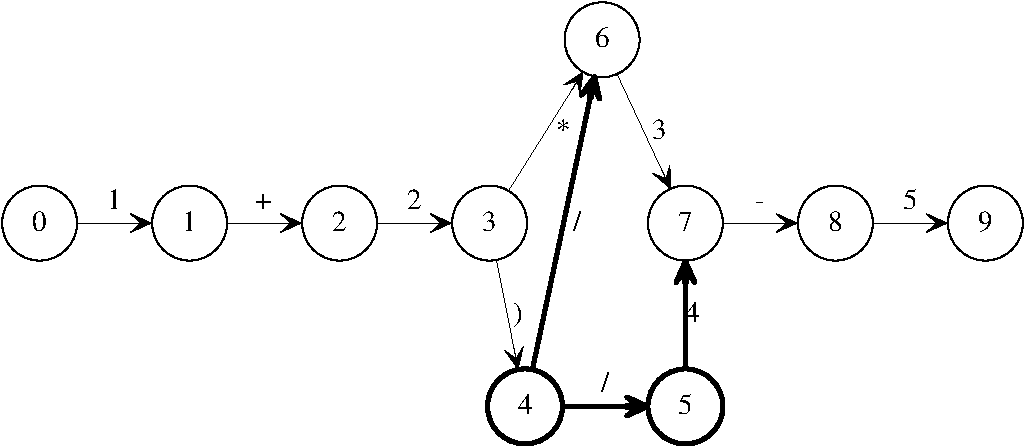
\includegraphics[width=\linewidth]{Verbitskaia/IgnoringPaths.pdf}
 \caption{Пример игнорирования части путей после ошибки}
 \label{ignor}
\end{figure}

Как уже говорилось, алгоритм абстрактного синтаксического анализа обрабатывает 
входной граф, представленный списком вершин, отсортированным в топологическом 
порядке. Эта особенность немного усложняет механизм игнорирования ошибочных путей. 
В тот момент, когда алгоритм обнаружил ошибку во входе, происходит вычисление 
игнорируемого интервала вершин. Если есть отложенные операции push, то следующей 
вершиной, из которой должен быть продолжен анализ, является вершина с номером 
равным минимуму из номеров отложенных операций push. Если же отложенных операций 
push нет, то рассматриваем все вершины стеков, сравниваем номера уровней, на 
которые последует переход, берем минимальное из этих значений и продолжаем анализ 
из вершины с вычисленным номером. Такой подход позволяет пропустить только те 
части путей в графе, которые гарантированно не будут переиспользованы ни в одном 
корректном выражении. 

\subsection{Специфика работы GLR-алгоритма}
К сожалению в ходе работы выяснилось, что не все проблемы, связанные с обнаружением 
ошибок, могут быть разрешены. Вопросы обнаружения ошибок и восстановления после 
них в GLR-алгоритме синтаксического анализа плохо изучены~\cite{economopoulos2006generalised}. Переход от классического 
алгоритма к абстрактному только усугубляет ситуацию. Например, мы не можем отличить 
конфликты, специфичные GLR-алгоритму (Shift/Reduce и Reduce/Reduce), и добавленный 
псевдоконфликт Shift/Shift. В результате этого становится невозможно понять причину 
возникновения некорректного состояния в стеке. Если такая ситуация возникла в 
результате Shift/Shift конфликта, то необходимо сообщать об ошибке, ведь это 
означает, что одно из входных выражений некорректно. Иначе сообщать об ошибке 
стоит только если на всех верхушках стека наблюдается некорректное состояние. 

Рассмотрим входной граф, изображенный на рисунке~\ref{both}. Во время анализа закрывающейся 
скобки на ребре (2~$\to$~3) будет получено два состояния: корректное и некорректное, 
соответствующие двум разным путям в графе. Анализатор не знает природу возникновения 
ошибки. Типичный для GLR-алгоритмов механизм обнаружения об ошибке сигнализирует 
о ней, только если все состояния на всех вершинах стека некорректны. Если применять 
такую стратегию к рассматриваемому случаю, то сообщения об ошибке на закрывающейся 
скобке не будет произведено, анализ будет продолжен, и в его результате будут 
получены всего два синтаксических дерева для двух синтаксически корректных выражений. 
Данное поведение некорректно, ведь если ошибок обнаружено не было, то все выражения 
стоит считать корректными, и в результате должно быть получено не два, а четыре 
синтаксических дерева.

\begin{figure}[h]
 \label{both}
 \centering
 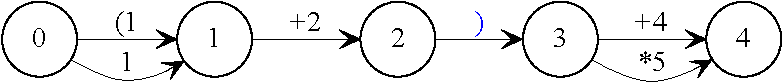
\includegraphics[width=0.75\linewidth]{Verbitskaia/BothStates.pdf}
 \caption{Входной граф с токеном, порождающим одновременно корректное и ошибочное состояние}
 \label{both}
\end{figure}

Текущая реализация алгоритма абстрактного синтаксического анализа сообщает обо 
всех случаях получения некорректного состояния в стеке. Таким образом, при обработке 
закрывающейся скобки будет диагностирована ошибка, но при этом все так же будут 
построены 2 корректных синтаксических дерева. 

Ситуация окажется намного сложнее при наличии разнородных конфликтов: если грамматика 
анализируемого языка неоднозначна, и входной граф при этом содержит множество 
ветвлений. В данной ситуации вероятно обнаружение большого количества ошибок, при 
этом не ясно, какие из срабатываний действительно соответствуют ошибкам во входных 
выражениях, а какие являются ложными и возникли вследствие неоднозначности грамматики. 

Одним из возможных решений проблемы было бы сохранение информации о характере 
конфликта и распространение ее вдоль всего пути. При таком подходе можно было бы 
определить исходную причину ошибки и выбрать, сообщать о ней или проигнорировать. 
Однако этот метод имеет ряд недостатков. Во-первых, все еще остается непонятным, 
что делать, если ошибка возникла где-нибудь после ветвления по конфликтам разного 
рода — и Shift/Shift, и Shift/Reduce или Reduce/Reduce. Во-вторых, даже если таких 
ситуаций не возникнет, распространение информации о характере ошибок потребует 
экспоненциальных ресурсов памяти. 

Стоит отметить, что если считать грамматику анализируемого языка однозначной, то 
есть не содержащей конфликтов типа Shift/Reduce и Reduce/Reduce, то обнаруживаемые 
ошибочные ситуации могут соответствовать только конфликтам ветвления. В данных 
условиях все обнаруженные ошибки будут соответствовать ошибкам во входных выражениях. 
Таким образом можно сказать, что если воспринимать текущую реализацию как расширение 
классического LR-алгоритма с использованием идей GLR-алгоритма, то нам известно 
как организовать механизм обнаружения ошибок. 

\subsection{Принципиально непорождаемые пути}
Помимо проблем, связанных непосредственно с обнаружением ошибок, есть еще и 
ограничения, связанные с аппроксимацией входного множества. Любая аппроксимация 
не точна, и в нашем случае может как не отражать всех возможных значений (например, 
при замене циклов на единственное повторение), так и порождать значения, которые 
никогда не могут быть сгенерированы во время работы анализируемой программы. 
Рассмотрим фрагмент кода, приведенный ниже. Граф, который будет сгенерирован по 
этому фрагменту кода и подан на вход анализатору, представлен на рисунке~\ref{instead}.

\begin{verbatim}
x = condition ? “(1+2” : “1+2”;
y = condition ? “)*3” : “*3”;
Program.Eval(y + x);
\end{verbatim}

\begin{figure}[h]
 \label{instead}
 \centering
 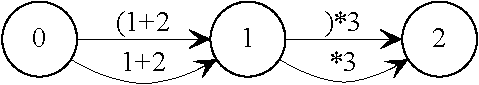
\includegraphics[width=0.5\linewidth]{Verbitskaia/4insteadOf2.pdf}
 \caption{Входной граф содержит четыре возможных пути}
 \label{instead}
\end{figure}

Легко заметить, что существует четыре пути во входном графе, соответствующие 
четырем различным выражениям, при этом среди них есть как синтаксически-корректные 
(первое и четвертое), так и некорректные (второе и третье).

\begin{enumerate}
    \item \begin{verbatim} “(1+2)*3”; \end{verbatim}
    \item \begin{verbatim} “(1+2*3”; \end{verbatim}
    \item \begin{verbatim} “1+2)*3”; \end{verbatim}
    \item \begin{verbatim} “1+2*3”. \end{verbatim}
\end{enumerate}

В силу использования одного и того же условия при выборе значения для составляющих 
частей динамически формируемого выражения, во время работы конечного приложения 
могут быть сгенерированны только первое и четвертое выражения, не содержащие 
синтаксических ошибок. Однако же реализованный абстрактный синтаксический анализатор 
проанализирует все четыре возможных варианта и сообщит об ошибках на открывающей 
и закрывающей скобке, так как они действительно имеются на двух возможных путях. 

С одной стороны, такое поведение является не совсем корректным, но на уровне 
синтаксического анализа мы ничего не знаем про общие условия и вообще природу 
возникновения тех или иных выражений, поэтому проблему обработки непорождаемых 
путей предлагается разрешить на этапе семантического анализа, во время которого 
мы обладаем всей необходимой для этого информацией. С другой стороны, нет ничего 
плохого в сообщении о большем количестве ошибок, чем есть на самом деле. В таком 
случае пользователь может обратить внимание на не самую хорошую структуру 
собственного кода и исправить ее.

% У заключения нет номера главы
\section*{Заключение}
В рамках данной работы были достигнуты следующие результаты.
\begin{itemize}
    \item Изучен механизм работы абстрактного RNGLR-алгоритма.
    \item Исследованы проблемы, связанные с обнаружением ошибок при абстрактном 
    анализе, основанном на RNGLR-алгоритме.
    \item На сколько это было возможно, в соответствии с результатами исследования, 
    был реализован механизм обнаружения ошибок во встроенных языках и сообщения о 
    них пользователю.
    \item Реализован набор тестов, фиксирующих полученный результат и демонстрирующих 
    недостатки.
\end{itemize}

Исходный код проекта YaccConstructor можно найти на сайте \cd{https://code.google.com/p/recursive-ascent}. 

В ходе работы было выявлено большое количество проблем, связанных с обнаружением 
ошибок в GLR-алгоритмах. При переходе к абстрактному алгоритму синтаксического 
анализа количество проблем увеличивается. Вопросы обнаружения и восстановления 
после ошибок гораздо лучше изучены для алгоритма обобщенного нисходящего анализа 
(Generalized Left-to-right Leftmost, GLL). В будущем планируется создание абстрактного 
синтаксического анализа, основанного на GLL-алгоритме. 

Отдельный вопрос, требующий внимательного изучения — необходимость использования 
восстановления после ошибок. Из-за усложнения алгоритмов самого анализа и диагностики 
ошибок восстановление может приводить к появлению большого числа ложных ошибок и 
только затруднять работу пользователя. С другой стороны, восстановление может 
оказаться полезным при использовании алгоритма в интегрированных средах разработки, 
используемых в интерактивном режиме.

\begin{thebibliography}{99}
\bibitem{Doh:2011:AL:2074591.2074599}
 Kyung-Goo Doh, Hyunha Kim, David A. Schmidt.
 Abstract LR-parsing // Formal Modeling, 2011.

\bibitem{Scott:2006:RNG:1146809.1146810}
 Elizabeth Scott, Adrian Johnstone.
 Right Nulled GLR Parsers //
 ACM Trans. Program. Lang. Syst, Vol.~28, \No~4, 2006.

\bibitem{Tomita:1984:LPN:980431.980564}
 Masaru Tomita.
 LR Parsers for Natural Languages //
 Proceedings of the 10th International Conference on Computational Linguistics, 1984.

\bibitem{Tomita:1985:ECP:1623611.1623625}
 Masaru Tomita.
 An Efficient Context-Free Parsing Algorithm for Natural Languages.
 Proceedings of the 9th International Joint Conference on Artificial Intelligence, 1985.

\bibitem{Tomita:1985:EPN:537456}
 Masaru Tomita.
 Efficient Parsing for Natural Language: A Fast Algorithm for Practical Systems. 
 Kluwer Academic Publishers, 1985.

\bibitem{economopoulos2006generalised}
  Giorgios Robert Economopoulos. 
  Generalised LR parsing algorithms. 2006.

\bibitem{rekers1992parser}
  Joan Gerard Rekers.
  Parser Gneration for Interactive Environments. 1992.

\bibitem{grigorev2013glr}
  Semen Grigorev, Iakov Kirilenko.
  GLR-based Abstract Parsing // 
  Proceedings of the 9th Central \& Eastern European Software Engineering Conference in Russia, 2013.

\bibitem{YaccConstructor}
 Кириленко Я.А., Григорьев С.В., Авдюхин Д.А.
 Разработка синтаксических анализаторов в проектах по автоматизированному реинжинирингу информационных систем //
 Научно-технические ведомости СПбГПУ. Информатика. Телекоммуникации. Управление, 2013.
\end{thebibliography}
